\documentclass[12pt]{article}
\usepackage[english]{babel}
\usepackage{natbib}
\usepackage{url}
\usepackage[utf8x]{inputenc}
\usepackage{amsmath}
\usepackage{graphicx}
\usepackage{subfig}
\graphicspath{{images/}}
\usepackage{parskip}
\usepackage{fancyhdr}
\usepackage{vmargin}
\usepackage{algorithm}
\usepackage[noend]{algpseudocode}
\newcommand{\var}{\texttt}
\usepackage[toc,page]{appendix}

\setmarginsrb{3 cm}{2.5 cm}{3 cm}{2.5 cm}{1 cm}{1.5 cm}{1 cm}{1.5 cm}

\title{Heuristics \& Approximations Algorithms}								% Title
\author{Alexander \& Narongrit}								% Author
\date{10 April 2019}											% Date

\makeatletter
\let\thetitle\@title
\let\theauthor\@author
\let\thedate\@date
\makeatother

\pagestyle{fancy}
\fancyhf{}
\rhead{\theauthor}
\lhead{\thetitle}
\cfoot{\thepage}

\makeatletter
\let\OldStatex\Statex
\renewcommand{\Statex}[1][3]{%
  \setlength\@tempdima{\algorithmicindent}%
  \OldStatex\hskip\dimexpr#1\@tempdima\relax}
\makeatother

\begin{document}

%%%%%%%%%%%%%%%%%%%%%%%%%%%%%%%%%%%%%%%%%%%%%%%%%%%%%%%%%%%%%%%%%%%%%%%%%%%%%%%%%%%%%%%%%

\begin{titlepage}
	\centering
    \vspace*{0.5 cm}
    
\includegraphics[scale = 0.5]{SDU_logo.png}\\[1.0 cm]	% University Logo
    \textsc{\LARGE University of Southern Denmark}\\[2.0 cm]	% University Name
	\textsc{\Large DM852}\\[0.5 cm]				% Course Code
	\rule{\linewidth}{0.2 mm} \\[0.4 cm]
	{ \huge \bfseries \thetitle}\\
	\rule{\linewidth}{0.2 mm} \\[1.5 cm]
	
	\begin{minipage}{0.4\textwidth}
		\begin{flushleft} \large
			\emph{Submitted To:}\\
			Marco Chiarandini\\
            Lene Monrad Favrholdt \\
			IMADA \\
			Mathematics \& Computer Science Department \\
			\end{flushleft}
			\end{minipage}~
			\begin{minipage}{0.4\textwidth}
            
			\begin{flushright} \large
			\emph{Submitted By :} \\
			Alexander Lerche Falk\\
            Narongrit Unwerawattana\\
            Spring - Master of Computer Science\\
		\end{flushright}
        
	\end{minipage}\\[2 cm]
	
	
    
    
    
    
	
\end{titlepage}

%%%%%%%%%%%%%%%%%%%%%%%%%%%%%%%%%%%%%%%%%%%%%%%%%%%%%%%%%%%%%%%%%%%%%%%%%%%%%%%%%%%%%%%%%

\tableofcontents
\pagebreak

%%%%%%%%%%%%%%%%%%%%%%%%%%%%%%%%%%%%%%%%%%%%%%%%%%%%%%%%%%%%%%%%%%%%%%%%%%%%%%%%%%%%%%%%%

\section{Introduction}

This project shows custom heuristic algorithms, resolving the Capacitated Vehicle Routing Problem (CVRP). When the heuristics have resolved the problem, given a canonical solution, we are applying custom \- and known \- Local Search algorithms to improve the results from the heuristics. 
The CVRP gives insight into how to deliver orders to customers using the shortest route for each vehicle, while preserving the capacity limit of each vehicle.\\
We have created two heuristic algorithms: one using a nearest-neighbour terminology and the other one taking inspiration of clustering close customers. We also show three custom developed Local Search algorithms. 
Lastly, we are going to compare our own ideas against more common used algorithms, which are tested and proved to work. 

\hspace{1 cm}--- Alexander \& Narongrit

\newpage

\section{Custom Heuristics Algorithms} 


The first algorithm, which we have created, takes the approach of the Nearest Neighbour idea. Given an instance of CVRP, the starting point - the depot where the vehicles are being loaded with customer requests - is the point, where all calculations begins. 
We start by checking the nearest point from the depot and add it to the first route. We then add next nearest point from the point recently added, and add it to the route. We continue until we are out of capacity, which is determined by each instance. We continue adding the nearest neighbour between the points until we have reached our capacity limit. At one point, we have covered all points, covering the problem instance, and giving us one or more routes for one or more vehicles.
The algorithm is described in pseudocode:
\newline

\begin{algorithm}[!ht]
	\caption{Custom CVRP Heuristic - Nearest Neighbour Approach}\label{euclid}
	\begin{algorithmic}[1]
	\Require{$Point_{1} \dots Point_{N}$} 
	\Ensure{$Solution$ (solution to the CVRP instance)}
	\Function{algorithm}{{$Points[\;]$}}
	\State $\var{capacity} \gets \text{0}$
	\State $\var{data} \gets \text{CVRP instance}$
	\State $\var{visited} \gets \textit{empty array containing visited nodes}$
	\State $\var{shortestdistance} \gets \textit{0}$
	\State $\var{current} \gets \textit{keep track of next node to visit}$
	\For{\texttt{$\var{i} \gets 0$ to $\text{length of data-1}$}}
		\For{\texttt{$\var{j} \gets 1$ to $\text{length of data}$}}
			\State $temp \gets \var{euclideandistance(\var{current}, \var{j})}$
			\If{$j$ not in $visited$}
				\If{$temp \leq shortestdistance$}
					\State $shortestdistance \gets temp$
					\State $current \gets j$
					\State $visited \gets j$
					\newline\Comment{checking if capacity requirements are met}
					\If{$\text{current total capacity} \leq \text{max capacity}$}
						\State $capacity \gets \text{capacity of current node}$					
					\Else
						\State $\text{Add starting point to end of route and}$
						\State $\text{add capacity of current node to variable(\var{capacity})}$
					\EndIf
				\EndIf
			\EndIf
		\EndFor
		\State $shortestdistance \gets 0$ \Comment{reset shortestdistance}
	\EndFor

	\State \textbf{return} $solution$
	\EndFunction
	\end{algorithmic}
\end{algorithm}

The first suggestion for an algorithm has a time complexity of $O(n^2)$. The algorithm has to iterate through the points of the instance twice. 
Given a point in the solution space, we are trying to find the shortest distance to any point from the current point. When we have found it, we are marking the point,
and making it the new current point. Then we continue to find the shortest distance to any non-visited point, while preserving the maximum capacity of the vehicle. 
At some point, we are out of space in the vehicle, leaving us no choice but to return to the depot. From here we start a new route until all points are visited.
\newline
Our next algorithm is inspired by Cluster Analysis \cite{website:cluster-analysis}, which is popular in machine learning and data mining. 
The idea is to group a set of points lying close to each other in an euclidean space. 
By choosing such approach to attack the CVRP, we can ensure points are lying close to each other before we are deriving a route.
\newline
The heuristic algorithm has the following behaviour: (1) Pick a customer point furthest from away from the depot, which is not in the solution route;
(2) Repeatly find nearest customer point from (1), which is not in any solution route and group such point together until the capacity is reached and save the points as a cluster; (3) Repeat (1) and (2) until we cover all customer points

The complexity of this algorithm is $O(n^2)$ since the main while loop terminates after we covered all customer points in a given instance. Furthermore each iteration in the while loop is executed in $O(n)$. 

\begin{algorithm}[!ht]
	\caption{Custom CVRP Heuristic - Clustering Approach}
	\begin{algorithmic}[1]
	\Require{$customers$: List of customer coordinate with it's capacity} 
	\Require{$depot$: Depot Point} 
	\Require{$maxcap$: Maximum capacity for each route} 
	\Ensure{$routes$: Solution to the CVRP instance}

	\State $\var{routes} \gets \textit{empty array containing solution routes}$
	\While{there is customer points not in solution}
		
	\State $\var{capacity} \gets \text{0}$
	\State $\var{route} \gets \text{[depot]}$
	
	\State $\var{startpoint} \gets$ furthest customer point from $\var{depot}$ which is not in solution
	\State add startpoint to route

	\State $\var{capacity} \gets \var{capacity} + \var{startpoint.capacity}$
		\While{$\var{capacity} < \var{maxcap} $}

			\State $\var{closest} \gets$ closest point from $\var{startpoint}$ not in solution

			\State $\var{c} \gets closest.capacity$

			\If{$\var{c} + \var{capacity} > \var{maxcap}$}
				\text{break}
			\EndIf
			\State $\var{capacity} \gets \var{capacity} + \var{c}$
			\State add closest to route
		\EndWhile
		\State add route to routes
	\EndWhile
	\State \textbf{return} $routes$
	\end{algorithmic}
\end{algorithm}
\newpage
\section{First Custom Local Search Algorithms}
Having executed the heuristics, providing us with solutions to the initial problem instances, we can continue optimizing. This is where the Local Search Optimization algorithms comes into play. 
Given a canonical solution, we want to optimize it to reduce the total cost of the solution. We have provided three custom Local Search (LS) algorithms, trying to optimize the canonical solution.
All of our localsearches optimize solution by make exchanges of visiting node between 2 routes in solution set. Thus they can be used in combination with original Traveling salesman problem's localsearches such as 2-opt and 3-opt, where improvements are done by swapping and reversing order of visiting nodes in single route.
\newline
The first LS algorithm looks into the generated routes done by the heuristics. It takes two routes and compare them with each other, checking if any swaps are possible in the two routes. 
A swap is possible if the distance is being reduced in at least one route, while still preserving the maximum capacity limit of both routes. 
The second LS algorithm looks like the first but with a minor change. It takes one route and compares it with every other route to find a better solution. It then continues doing this 
with every other route. 

\section{Second Custom Local Search Algorithms} \label{ls2}
This localsearch algorithm for CVRP is inspired from the fact that if we wanted to find a customer point to move from one route to another, such point has to be the point that form a convex hull of the route. We developed an algorithm to reduce the number of comparisons done by each iteration on each route by computing the convex hull points of each route, and only use those point as candidates for interchanging points in the routes. 
We also gain the benefit from haveing such list to estimate a "central" of the route by computing the average of convex hull point. We use the central point as the reference point of a route to find the closest point in others. These points are visualized in the figure, where lines are convex hull of a route. Point \(A\) and \(B\) are the closest points to central point from route \(i\) to route \(j\) (\(mid\_j\)) and from route \(j\) to \(i\) (\(mid\_i\)) respectively.

\begin{figure}[H]
	\caption{Convex hull points and central points of two routes}
	\centering
	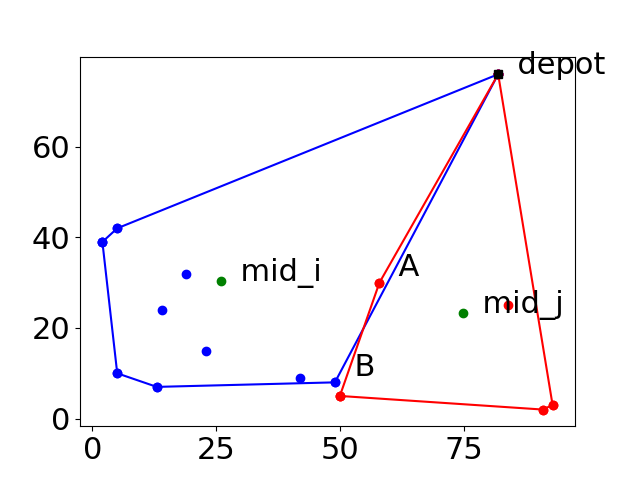
\includegraphics[width=0.5\textwidth]{convexmidclosest.png}
	\label{fig:localsearch1}

\end{figure}


We implemented an algorithm defined by Mark de Berg \cite{Berg97} which has a runtime complexity of $O(nlogn)$. Our local search is given by a pair of routes: namely \(i\) and \(j\). We find the closest point from route \(i\) to \(j\) by comparing the central points in the convex \(i\) to the central point of the convex \(j\) and closest point from \(j\) to \(i\) respectively. 
The possibilities of interchanging point from route \(i\) to \(j\) are defined in the following three cases:
\begin{enumerate}

	\item If the capacity constraint from moving \(i\) to \(j\) does not exceed its maximum, we compare if moving the closest customer point from \(i\) to \(j\) generates a better route. If so, we proceed and move the point from \(i\) to \(j\)

	\item If the capacity constraint from moving \(j\) to \(i\) does not exceed its maximum, we compare if moving the closest customer point from \(j\) to \(i\) generates a better route. If so, we proceed and move the point from \(j\) to \(i\)

	\item if the capacity constraint from swapping the closest customer point of \(i\) to \(j\) does not exceed, we compare if swapping the points of the two routes generates a better route. If so, we swap the candidate point from route \(i\) to route \(j\) and \(j\) to \(i\) respectively.
\end{enumerate}

When we are performing  the moving cases (1 and 2), we should also take into account the tour order. This is shown in figure \ref{fig:local_case1}
\newline

\begin{figure}[!ht]
	\centering
	\subfloat[Move Case]{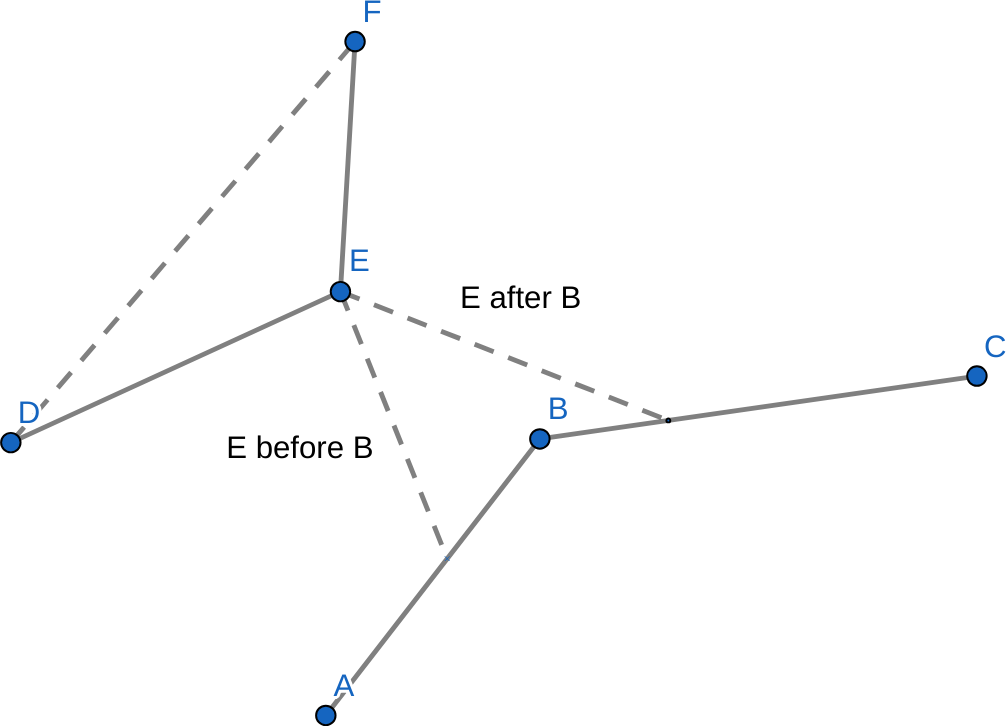
\includegraphics[width=0.4\textwidth]{movepointtoroute.png}\label{fig:local_case1}}
	\hfill
	\subfloat[Swap Case]{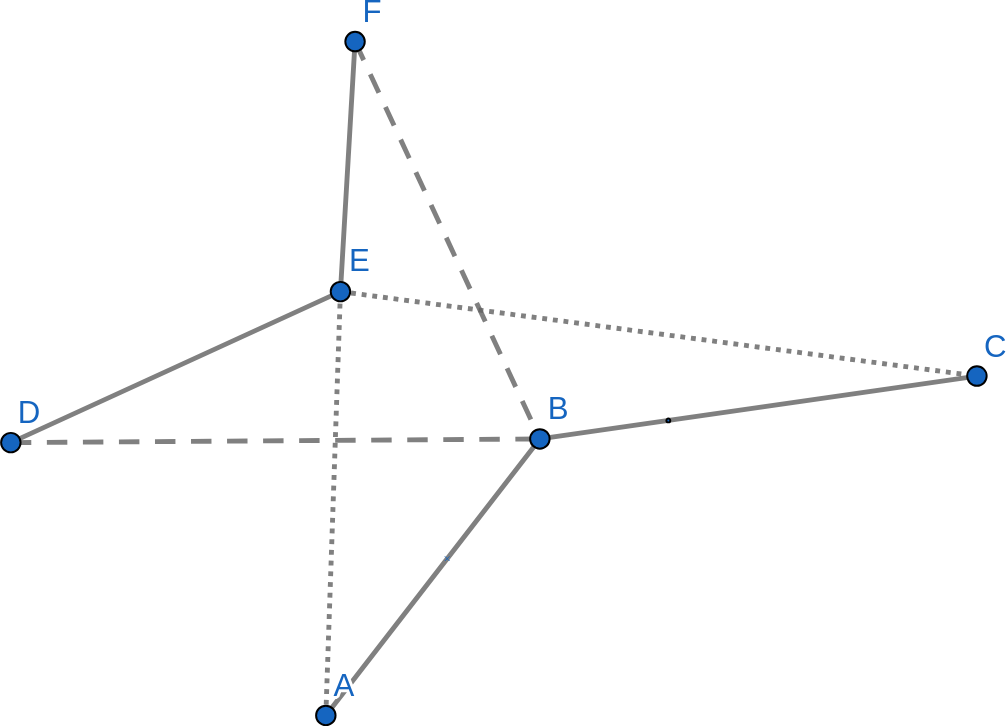
\includegraphics[width=0.4\textwidth]{swapcase.png}\label{fig:local_case2}}
\end{figure}

Moving point E - which is the closest point in route \(j\)to \(i\) - is resulted in a different tour between visiting E before \(B\) or after. Thus, it is necessary to compare cost between these two sub cases before performing the move operation as shown Appendix C, Line 9. The complexity is $O(n^2)$ and all operations inside the loop have the complexity of at most $O(n)$. If we have the improvement of route, we recompute the convex hull of 2 routes, thus, the complexity of each iteration of this localsearch is at most $O(n^3logn)$

\section{Performance Analysis \& Boxplots}
It has been a challenge to come up with our own custom solutions. The results we got from our algorithms and experiments
were good, but we do see struggles in our design. An example of this is shown in the NN algorithm, where the first couple of routes are good, but then the later have longer distances between the points, because they are "leftovers". 
\newline
Our algorithms were built without trying to be biased towards other existing algorithms. We tried to use our own imagination on how the problems could be solved. 
We have been inspired by concepts but not algorithms directly, and it has made us more aware on how to tackle problems and how not to.
\newline
We have tried to create boxplots for our custom algorithms to give an indication whether or not the algorithms performs somewhat similar on the same instance, but with 
a bigger dataset. Meaning: it is not completely random, even though the instance looks the same but has more data. If you look at the boxplot of our custom "close-index" local search algorithm - Figure \ref{fig:custom_close_idx_localsearch_boxplot_fig_cluster} - applied on the heuristic cluster algorithm
and compare it to the two-opt local search algorithm - Figure \ref{fig:two_opt_cluster} - applied on the same heuristic, then you are able to see the two-opt does better - especially on the golden instances - but on the other instances, we are getting there. 
\newline 
\textit{All the boxplots can be found in the appendices.}
\newline



\section{Process Analysis}
The group work went well. We were both enthusiastic about the work and wanted to try out as much as possible. 
The communication between us has been nice and we have been splitting out the work in somewhat equal pieces to adapt to the workload from other courses.

Alexander Lerche Falk
\begin{itemize}
	\item Develop Nearest Neighbour Approach Heuristric \item Develop Custom Local Search Algorithms 1
	\item Performance analysis of Heuristics and Localsearchs
\end{itemize}
Narongrit Unwerawattana
\begin{itemize}
	\item Develop Clustering Approach Heuristic
	\item Develop Custom Local Search Algorithms 2
	\item Develop 2 and 3 opt localsearch
\end{itemize}
both
\begin{itemize}
	\item Writing report
\end{itemize}


\newpage
\bibliographystyle{plain}
\bibliography{references}

\newpage
\begin{appendices}

\section{\\Custom Cluster Algorithm to solve CVRP}
% the \\ insures the section title is centered below the phrase: AppendixA

\begin{algorithm}[!ht]
	\caption{Cluster CVRP Localsearch}
	\begin{algorithmic}[1]
	\Require{$closest\_point(A, points)$: returns point in points which hase minimum distance from A} 
	\Require{$elim\_empty\_routes$: returns list of routes where the empty routes are removed}
	\Ensure{$routes$: Better Solution to the CVRP instance}
	\Function{algorithm}{{$routes$, $maxcap$}}
	\State $\var{route\_convexes}$ is an array storing convex\_hull for each route  
	\State $\var{improvements} \gets \text{True}$
	\While{\texttt{$\var{improvements}$}}
		\ForAll{$i$, $j$ such that $i$, $j$ are routes index combination}
			\State $\var{central\_point\_i} \gets$ average of point in convex i

			\State $\var{central\_point\_j} \gets$ average of point in convex j
			
			\State $\var{closest\_from\_i\_j} \gets \text{closest\_point(mid\_point\_i, convex\_routes[j])}$

			\State $\var{closest\_from\_j\_i} \gets \text{closest\_point(mid\_point\_j, convex\_routes[i])}$

			\If{$\var{closest\_from\_i\_j}$ and $\var{closest\_from\_j\_i}$ is Found}
			
			\If{$closest\_from\_i\_j$ fits in route j}
				\State \text{add move to route improvements j}
				\State \text{make the swap}
			\ElsIf{$closest\_from\_j\_i$ fits in route i}
				\State \text{add move to route improvements i}
				\State \text{make the swap}
			\ElsIf{capacity is not reached by swapping customers}
				\State \text{swap the route-points between i and j}
			\EndIf

			\If{$\var{improvements}$}
				\State recalculate convex hull of route i and j				
			\EndIf
			\EndIf
			\EndFor

		\If{\textbf{not} $\var{improvements}$}
			\State $\var{routes} = elim\_empty\_routes(\var{routes})$
			\Return $\var{routes}$
		\EndIf
	\EndWhile
	\EndFunction

	\end{algorithmic}
\end{algorithm}

\section{\\LocalSearch Algorithm - Swap if any improvement}

\begin{algorithm}[!ht]
	\caption{swap\_if\_improvement}
	\begin{algorithmic}[1]
		\Require{$dist(A,B)$ returns distance from point A to B}
	\Function{swap\_if\_improvement}{{$route\_i, route\_j, j\_to\_i, i\_to\_j$}}

	\State $\var{A}, \var{B}, \var{C} \gets \var{route\_i[i\_to\_j-1]}, \var{route\_i[i\_to\_j]},$
	\Statex $\var{route\_i[i\_to\_j+1 mod(\%) len(route\_i)]}$
	\State $\var{D}, \var{E}, \var{F} \gets \var{route\_j[j\_to\_i-1]}, \var{route\_j[j\_to\_i]},$ 
	\Statex $\var{route\_j[j\_to\_i+1 mod(\%) len(route\_j)]}$

	\State $\var{old\_distance\_i} \gets dist(\var{A},\var{B}) + dist(\var{B},\var{C})$
	\State $\var{old\_distance\_j} \gets dist(\var{D},\var{E}) + dist(\var{E},\var{F})$

	\State $\var{new\_distance\_i} \gets dist(\var{A},\var{E}) + dist(\var{E},\var{C})$
	\State $\var{new\_distance\_j} \gets dist(\var{D},\var{B}) + dist(\var{B},\var{F})$

	\If{$\var{old\_distance\_i} + \var{old\_distance\_j} >$ 
		\Statex $\var{new\_distance\_i} + \var{new\_distance\_j}$}
		\Statex $\text{swap point B of route i with point E of route j}$
		\Statex \Return True
	\EndIf
	\EndFunction

	\end{algorithmic}
\end{algorithm}

\newpage
\section{\\LocalSearch Algorithm - Move if any improvement}

\begin{algorithm}[!ht]
	\caption{move\_if\_improvement}
	\begin{algorithmic}[1]
		\Require{$dist(A,B)$ returns distance from point A to B}
	\Function{move\_if\_improvement}{{$route\_i, route\_j, i\_to\_j, j\_to\_i$}}

	\State $\var{A}, \var{B}, \var{C} \gets \var{route\_i[i\_to\_j -1]}, \var{route\_i[i\_to\_j]},$
	\Statex $\var{route\_i[i\_to\_j+1 \% len(route\_i)]}$

	\State $\var{D}, \var{E}, \var{F} \gets \var{route\_j[j\_to\_i -1]}, \var{route\_j[j\_to\_i]},$ 
	\Statex $\var{route\_j[j\_to\_i+1 \% len(route\_j)]}$


	\State $\var{old\_distance\_i} \gets dist(\var{A},\var{B}) + dist(\var{B},\var{C})$
	\State $\var{old\_distance\_j} \gets dist(\var{D},\var{E}) + dist(\var{E},\var{F})$

	\State $\var{new\_dist\_before\_B} \gets dist(\var{A},\var{E}) + dist(\var{E},\var{B}) + dist(\var{B},\var{C})$ 

	\State $\var{new\_dist\_after\_B} \gets dist(\var{A},\var{B}) + dist(\var{B},\var{E}) + dist(\var{E},\var{C})$ 

	\State $\var{new\_distance\_j} \gets dist(\var{D},\var{F})$

	\If{$\var{new\_dist\_before\_B} < {new\_dist\_after\_B}$}

		\If{$\var{old\_distance\_i} + \var{old\_distance\_j} >$ 
			\Statex $\var{new\_dist\_before\_B} + \var{new\_distance\_j}$}
			\Statex $\text{move point E from route j to route i before B}$
		\EndIf
	\Else

		\If{$\var{old\_distance\_i} + \var{old\_distance\_j} >$ 
			\Statex $\var{new\_dist\_after\_B} + \var{new\_distance\_j}$}
			\Statex $\text{move point E from route j to route i after B}$

		\EndIf
	\EndIf
	\EndFunction

	\end{algorithmic}
\end{algorithm}

\section{\\ BOXPLOT FIGURES}

\begin{figure}
	\centering
	\caption{Heuristic NN Algorithm - Custom}{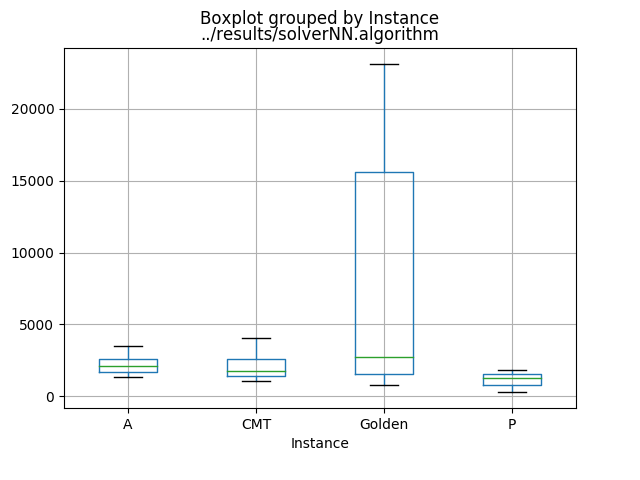
\includegraphics[width=0.8\textwidth]{solverNN_algorithm_boxplot.png}\label{fig:NN_heuristic_fig}}
\end{figure}

\begin{figure}[!htb]
	\centering
	\caption{Heuristic Cluster Algorithm - Custom}{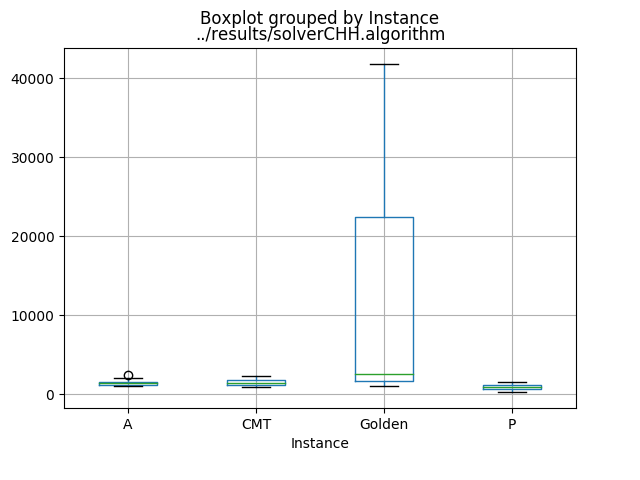
\includegraphics[width=0.8\textwidth]{solverCHH_algorithm_boxplot.png}\label{fig:Cluster_heuristic_fig}}
\end{figure}

\begin{figure}[!htb]
	\centering
	\caption{Local Search Algorithm - Custom - Close index route for NN heustic}{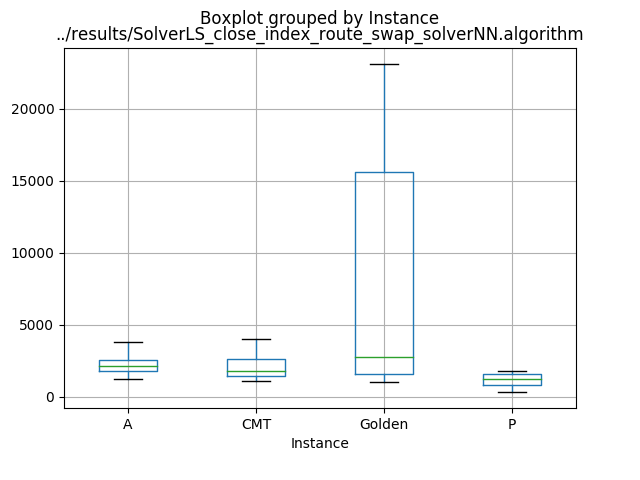
\includegraphics[width=0.8\textwidth]{SolverLS_close_index_route_swap_solverNN_algorithm_boxplot.png}\label{fig:custom_close_idx_localsearch_boxplot_fig_nn}}
\end{figure}
\begin{figure}[!htb]
	\centering
	\caption{Close Index Custom Local Search Figure for cluster heuristic}{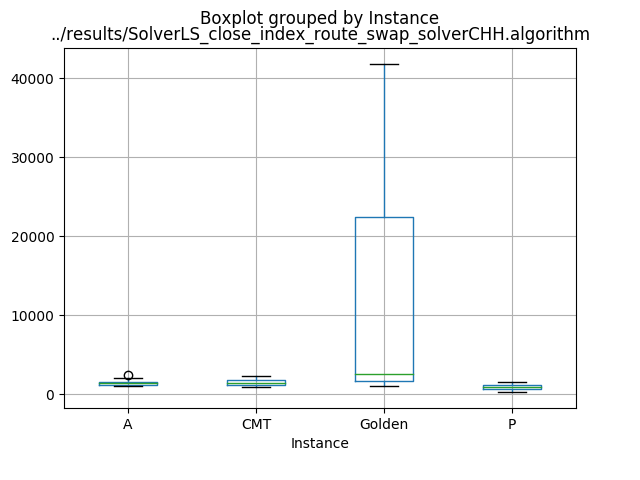
\includegraphics[width=0.8\textwidth]{SolverLS_close_index_route_swap_solverCHH_algorithm_boxplot.png}\label{fig:custom_close_idx_localsearch_boxplot_fig_cluster}}
\end{figure}

\begin{figure}[!htb]
	\centering
	\caption{Local Search Algorithm - Custom - All index combinations route for NN heuristic}{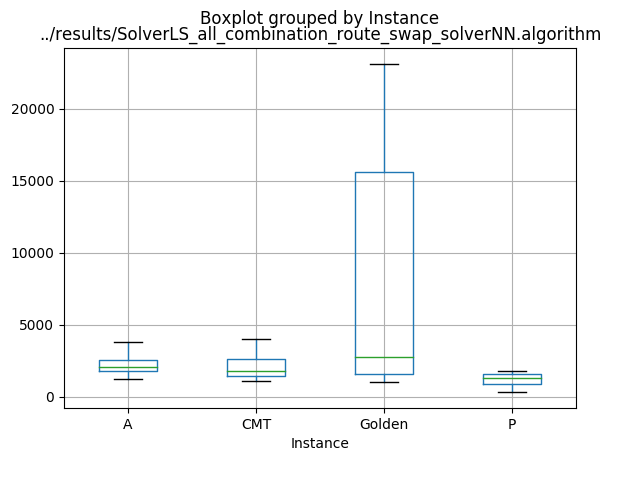
\includegraphics[width=0.8\textwidth]{SolverLS_all_combination_route_swap_solverNN_algorithm_boxplot.png}\label{fig:all_combinations_localsearch_boxplot_fig_nn}}
\end{figure}
\begin{figure}[!htb]
	\centering
	\caption{Local Search Algorithm - Custom - All index combinations route for cluster heuristic}{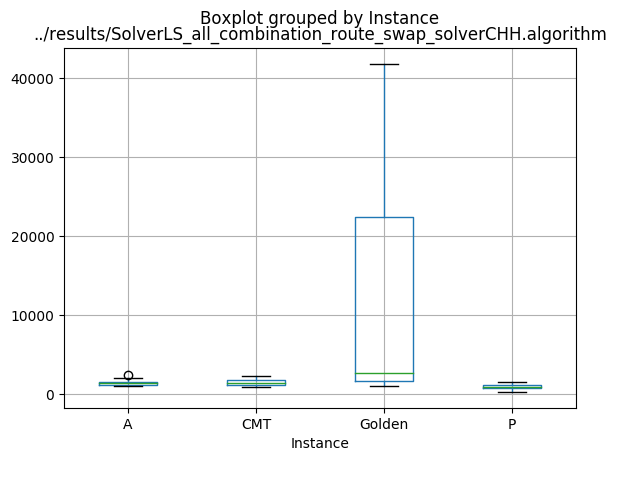
\includegraphics[width=0.8\textwidth]{SolverLS_all_combination_route_swap_solverCHH_algorithm_boxplot.png}\label{fig:all_combinations_localsearch_boxplot_fig_cluster}}
\end{figure}

\begin{figure}[!htb]
	\centering
	\caption{Local Search Algorithm - Known - Two Opt for NN heuristic}{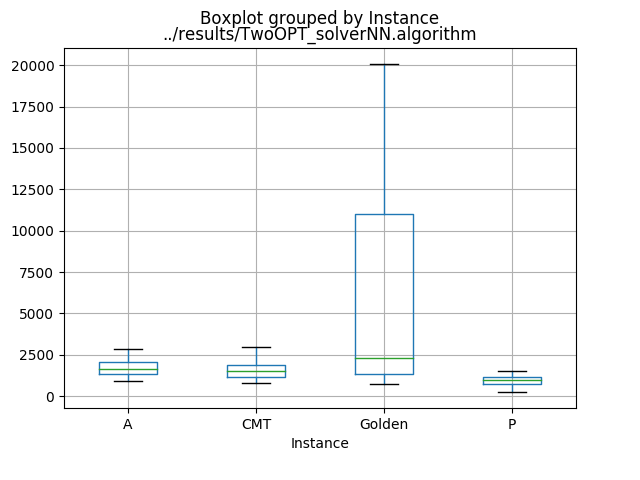
\includegraphics[width=0.8\textwidth]{TwoOPT_solverNN_algorithm_boxplot.png}\label{fig:two_opt_nn}}
\end{figure}
\begin{figure}[!htb]
	\centering
	\caption{Two Opt Known Local Search Figure for cluster heuristic}{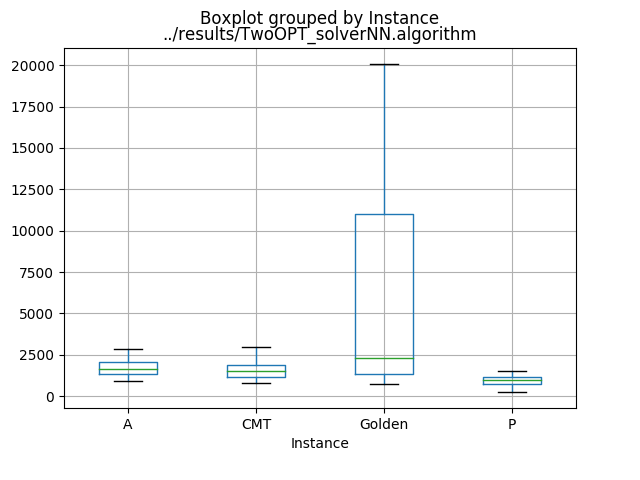
\includegraphics[width=0.8\textwidth]{TwoOPT_solverNN_algorithm_boxplot.png}\label{fig:two_opt_cluster}}
\end{figure}

\end{appendices}
\end{document}